\chapter{Methods}


\section{Data}
This work relies on two types of data, the ground truth, the measured irradiance at the power station and the input, the irradiance values from high-resolution weather forecasts for the area. The data used spans the 425 days from August 1 2020 to September 30 2021 for the Ituverava solar power station run by Enel S.p.A. in Minas Gerais, Brazil.

\subsection{Irradiance measurements}
The irradiance was measured with seven Kipp \& Zonen CM21 pyranometers placed around the power station. The pyranometers have a reported maximum measurement error of 3\%. For input into the network, the highest and lowest measured values are dropped and the average value of the other five measurements is used. This data is provided with five-minute intervals, but the neural network operates hourly. To downsample the measurement data to an hourly format, we averaged the values for the twenty minutes before and after the top of each hour. Finally, the irradiance values were normalized linearly to the range 0-1 before input into the neural network.
\newpage

\subsection{Forecast Data}
The weather forecast data is provided by Belgingur ehf., Reykjavik, Iceland. We use irradiance values from historical 24-hour weather forecasts generated by their WRF model, discussed in section~\ref{cha:WRF}. The forecasts have a temporal resolution of one hour and a spatial resolution of 2.5km. One of our models uses forecast data from a 3x3 grid centred on the solar power station, and the other model only the data from the centre of the grid. We use two irradiance values from the forecast, the downward irradiance and the downward diffuse irradiance. These irradiance values were normalized linearly to the range 0-1 before input into the neural network.


\subsubsection{Data Source}\label{cha:WRF}
\textcolor{red}{TODO: Talk about WRF} \cite{gueymard_global_2008, rognvaldsson_numerical_2013, jimenez_wrf-solar_2016}


\subsection{Error metric}
In other work done in this area, multiple error metrics are used. One error metric is used more commonly than others, Mean Absolute Percentage Error (MAPE) \cite{lin_temporal_2020, lee_forecasting_2018, jaidee_very_2019, su_machine_2019}, which is the reason that metric was chosen.
When working with near-zero values MAPE becomes unhelpful as it is calculated by dividing by that near-zero value, so all cases where the irradiance is less than 15\% of the maximum value in the data set are dropped. Hence we do not evaluate early morning or late evening performance.
While a valuable metric, MAPE does not  fully represent the value of the model. Other factors like confidence, discussed in section~\ref{sec:loss_function} and deviance from total irradiance for the day also represent key factors in the usefulness of the model.

\newpage


\section{Tools}
The neural network was implemented in PyTorch 1.11 and PyTorch Forecasting 0.9.0. We used an NVIDIA GeForce RTX 3080Ti graphics card using CUDA for training. The computer had an AMD Ryzen 9 5950X CPU, 32GB of RAM and was running Windows 11.
This allowed for quick training of models, as with the relatively small amount of data, training a model took 5-10 minutes.


\newpage
\section{Model}
    \subsection{Temporal Fusion Transformer}
    \textcolor{red}{TODO}
    \cite{lim_temporal_2020}
    
    \begin{figure}[ht!]
        \centering
        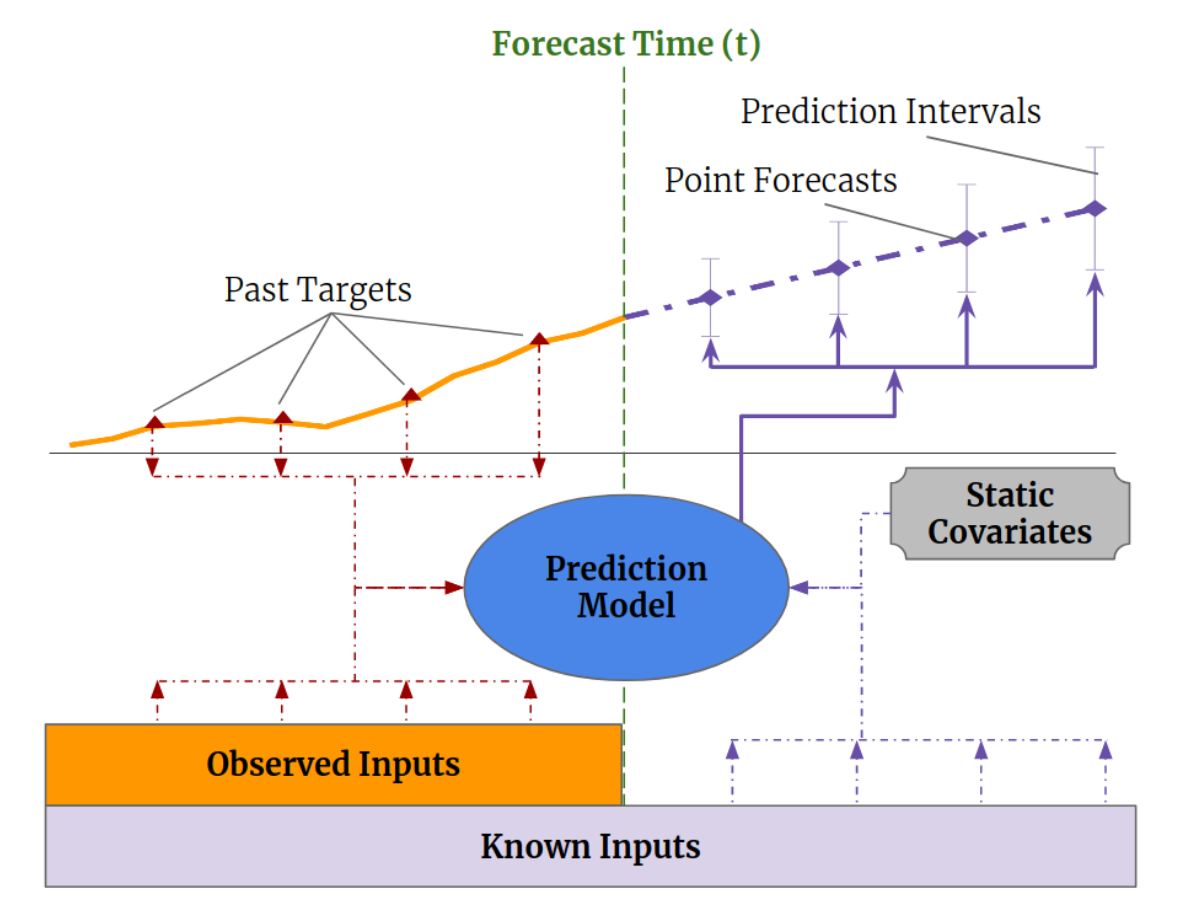
\includegraphics[scale=0.4]{imgs/TFT1.png}
        \caption{An overview of the Temporal Fusion Transformer.\cite{lim_temporal_2020}
        \label{fig:tft_overviwew}}
    \end{figure}
\newpage
    \begin{figure}[ht!]
        \centering
        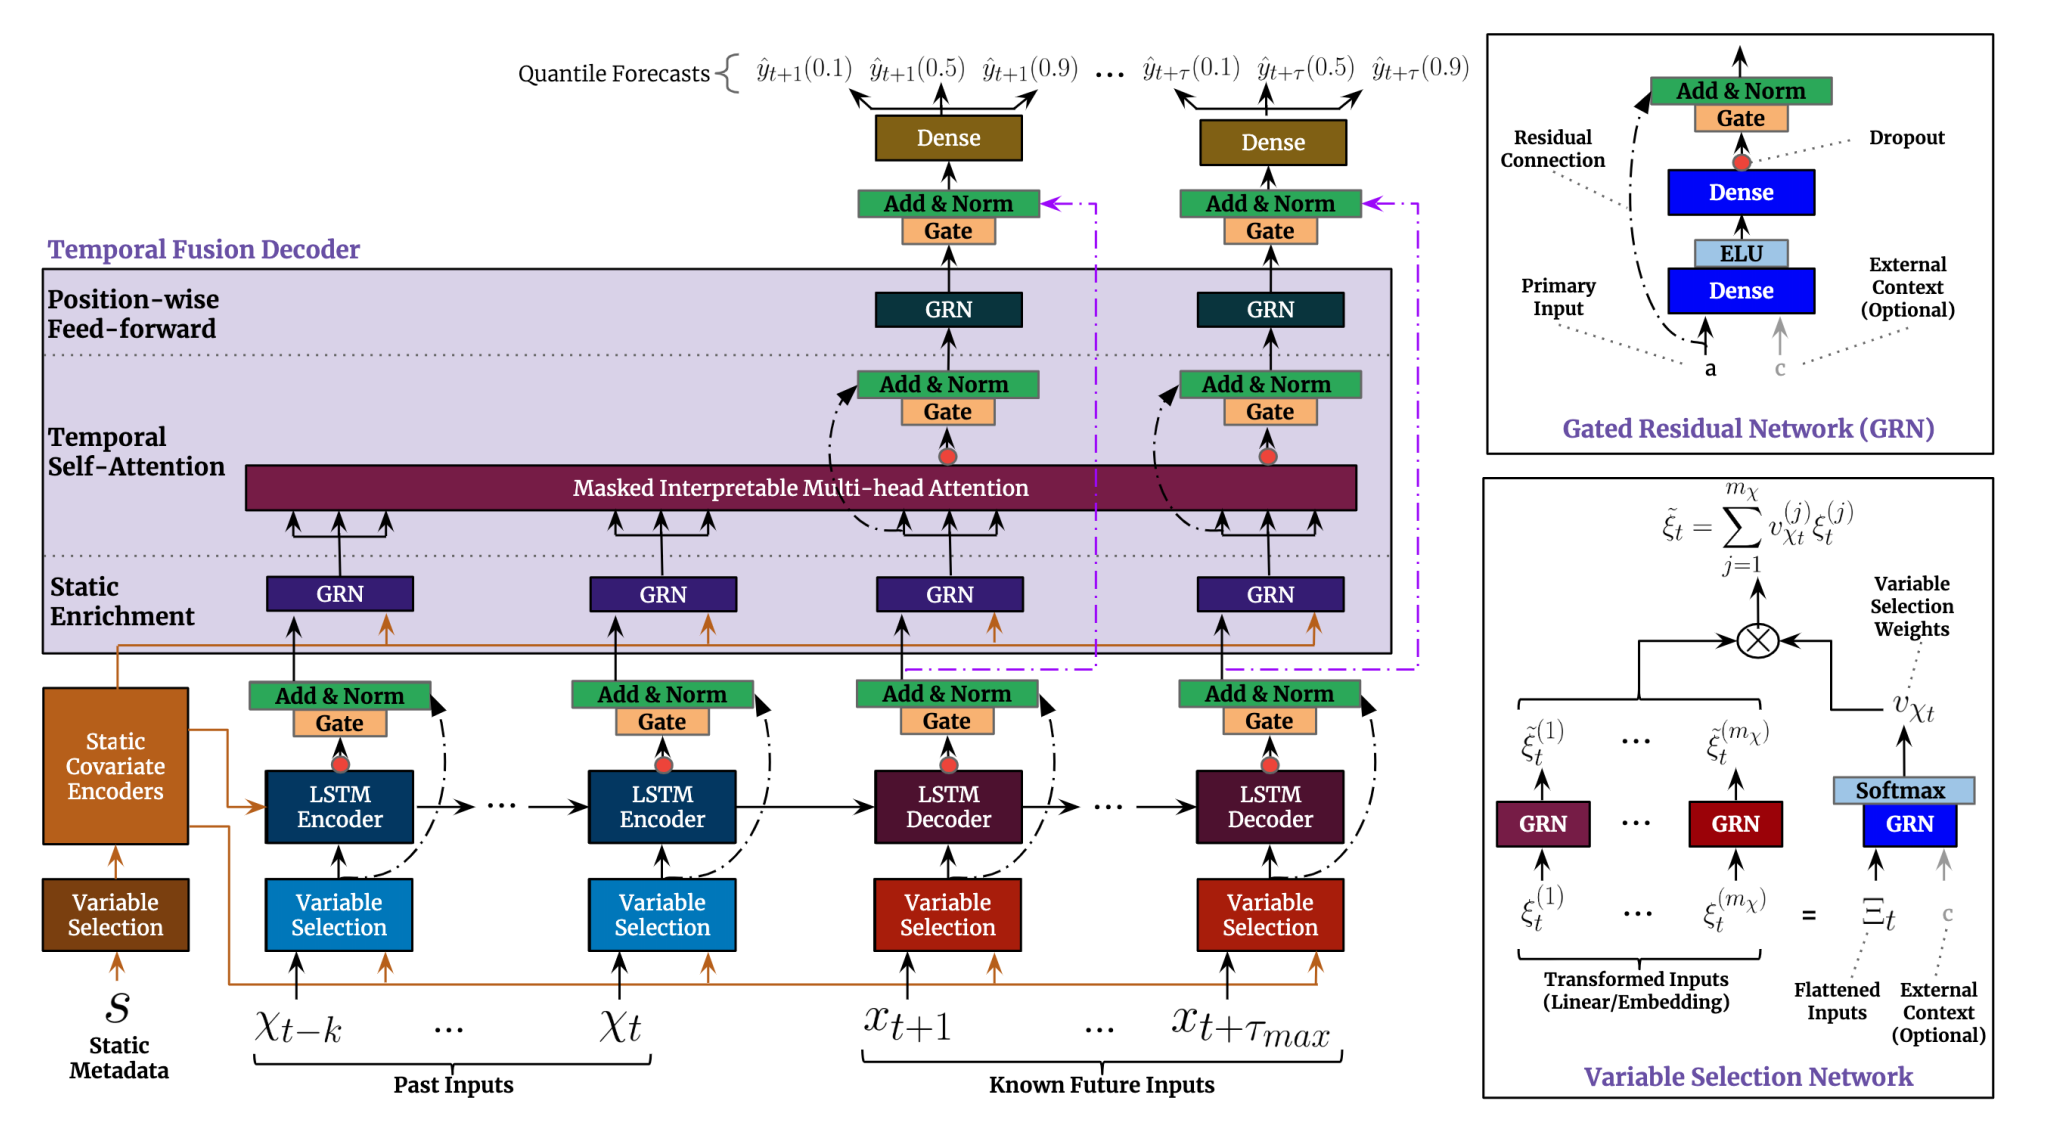
\includegraphics[scale=0.27]{imgs/TFT.png}
        \caption{A detailed view of the architecture of the Temporal Fusion transformer.\cite{lim_temporal_2020}
        \label{fig:ttgt_detail}}
    \end{figure}
    
    
    \newpage
    \subsection{Setup}
    \textcolor{red}{TODO}
    
        \begin{table}[ht!]
        \begin{center}
        \caption{The full model hyperparameters.
        \label{tab:full_params}}
        \vspace{0.5cm}
        \begin{tabular}{|l|l|}
        \hline
        \textbf{Hyperparameter} & \textbf{Value} \\ \hline
        Learning rate            & 0.01         \\ \hline
        Batch size              & 24            \\ \hline
        Dropout                 & 0.1            \\ \hline
        Hidden size            & 64         \\ \hline
        Hidden continuous size & 8         \\ \hline
        Attention head size    & 1         \\ \hline
        \end{tabular}
        
        \end{center}
        \end{table}
        
        \begin{table}[ht!]
        \begin{center}
        \caption{The limited model hyperparameters.
        \label{tab:lim_params}}
        \vspace{0.5cm}
        \begin{tabular}{|l|l|}
        \hline
        \textbf{Hyperparameter} & \textbf{Value} \\ \hline
        Learning rate            & 0.005         \\ \hline
        Batch size              & 24            \\ \hline
        Dropout                 & 0.1            \\ \hline
        Hidden size            & 40         \\ \hline
        Hidden continuous size & 6         \\ \hline
        Attention head size    & 1         \\ \hline
        \end{tabular}
        
        \end{center}
        \end{table}
    
    \subsubsection{Loss function}\label{sec:loss_function}
    \textcolor{red}{TODO: Fix, find more sources and make sure this is correct}\\
    We use the quantile loss  Temporal Fusion Transformers is quantile loss, which we use.
    A model's prediction is a random value within a probability distribution \cite{}. If we make multiple predictions we can estimate this probability distribution by seeing within what range a selected proportion of the predictions fall \cite{koenker_quantile_2001}. PyTorch Forecasting's quantile loss function takes the Mean Absolute Error (MAE) of three quantiles, 90\%, 50\% and 10\%. [0.02, 0.1, 0.25, 0.5, 0.75, 0.9, 0.98] This gives a good picture of the model's confidence in a prediction. A smaller quantile range indicated more confidence.
    